2.2 պարագրաֆում $W(G\square H)$-ի հայտնի գնահատականը լավացվել է այն դեպքում, երբ գրաֆներից մեկը համասեռ է: 

\begin{theorem}
\label{t2_regular_product} Եթե $G,H\in \mathfrak{N}$, ընդ որում $H$-ը $r$-համասեռ է, ապա.
\begin{center}
$W(G\square H)\geq W(G)+W(H)+r$:
\end{center}
\end{theorem}
\begin{proof}[Ապացույց]
Դիցուք $\alpha$-ն $G$ գրաֆի կողային միջակայքային $t_G$-ներկում է, իսկ $\beta$-ն $H$ գրաֆի միջակայքային $t_H$-ներկում է: Թեորեմն ապացուցելու համար բավական է կառուցել $G\square H$ գրաֆի համար $\gamma$ միջակայքային ներկում՝ $t_G+t_H+r$ գույներով: 

Առանց ընդհանրությունը խախտելու կարող ենք ենթադրել, որ $\underline{S}(u_1,\alpha)=1$, $\underline{S}(v_1,\beta)=1$, $\overline{S}(u_m,\alpha)=t_G$ և $\overline{S}(v_n,\beta)=t_H$: $\gamma$ ներկումը սահմանենք հետևյալ կերպ.
\begin{description}
\item[(1)] $\gamma\left((u_i,x)(u_i,y)\right) = \beta(xy) + \underline{S}(u_i,\alpha) - 1$, որտեղ $xy \in E(H)$ և $i=1,\ldots,m-1$
\item[(2)] $\gamma\left((x,v_j)(y,v_j)\right) = \alpha(xy) + \overline{S}(v_j,\beta)$, որտեղ $xy \in E(G)$ և $j=1,\ldots,n$
\item[(3)] $\gamma\left((u_m,x)(u_m,y)\right) = \beta(xy) + \overline{S}(u_m,\alpha) + r$, որտեղ $xy \in E(H)$
\end{description}
Այսպիսի ներկման դեպքում արտադրյալ գրաֆի գագաթների սպեկտրները կլինեն.
\begin{align*}
S\left( (u_i,v_j) \right) &= \left[ \underline{S}(v_j,\beta) + \underline{S}(u_i,\alpha) - 1, \overline{S}(v_j,\beta) + \underline{S}(u_i,\alpha) - 1 \right] \cup \\
&\cup \left[ \underline{S}(u_i,\alpha) + \overline{S}(v_j,\beta), \overline{S}(u_i,\alpha) + \overline{S}(v_j,\beta) \right] = \\
&= \left[ \underline{S}(v_j,\beta) + \underline{S}(u_i,\alpha) - 1, \overline{S}(u_i,\alpha) + \overline{S}(v_j,\beta) \right]\\
&i=1,\ldots,m-1\ \ j=1,\ldots,n\\
S\left( (u_m,v_j) \right) &= \left[ \underline{S}(u_m,\alpha) + \overline{S}(v_j,\beta), \overline{S}(u_m,\alpha) + \overline{S}(v_j,\beta) \right] \cup \\
&\cup \left[ \underline{S}(v_j,\beta) + \overline{S}(u_m,\alpha) + r, \overline{S}(v_j,\beta) + \overline{S}(u_m,\alpha) + r \right] = \\
&= \left[ \underline{S}(u_m,\alpha) + \overline{S}(v_j,\beta) , \overline{S}(v_j,\beta) + \overline{S}(u_m,\alpha) + r \right]\\
&j=1,\ldots,n
\end{align*}
Վերջին հավասարությունը տեղի ունի, քանի որ $H$ գրաֆի համասեռությունից՝ $\overline{S}(v_j,\beta) - \underline{S}(v_j,\beta) = r - 1$: Նկատենք, որ $\underline{S}(u_1,v_1)=\underline{S}(v_1,\beta)+\underline{S}(u_1,\alpha)-1=1$ և $\overline{S}(u_m,v_n)=\overline{S}(v_n,\beta)+\overline{S}(u_m,\alpha)+r=t_G+t_H+r$: Հետևաբար, Լեմմա \ref{t1_lemma}-ից՝ $\gamma$-ն $G \square H$ գրաֆի միջակայքային $(t_G+t_H+r)$-ներկում է:
\end{proof}
\begin{hide}
\begin{corollary}
\label{t2_regular_product_2}
Եթե $G,H\in \mathfrak{N}$, ընդ որում $G$-ն $r$-համասեռ է, իսկ $H$-ը՝ $r'$-համասեռ, ապա $W(G\square H)\geq W(G)+W(H)+\max{\left\{r,r'\right\}}$:
\end{corollary}
\begin{corollary}
\label{t2_regular_k_product} 
Դիցուք $G_1, G_2, \ldots, G_k \in \mathfrak{N}$, $G_i$-ն $r_i$-համասեռ է, $i=1,\ldots,k$, ընդ որում $r_1\geq r_2\geq \ldots \geq r_k$: Այդ դեպքում.
\begin{center}
$W(G_1 \square G_2 \square \ldots \square G_k) \geq \sum\limits_{i=1}^{k}W(G_i) + \sum\limits_{i=1}^{k-1}{\sum\limits_{j=1}^{i}{r_j}}$
\end{center}
\end{corollary}
\end{hide}

\begin{hide}
\begin{figure}[t]
\centering
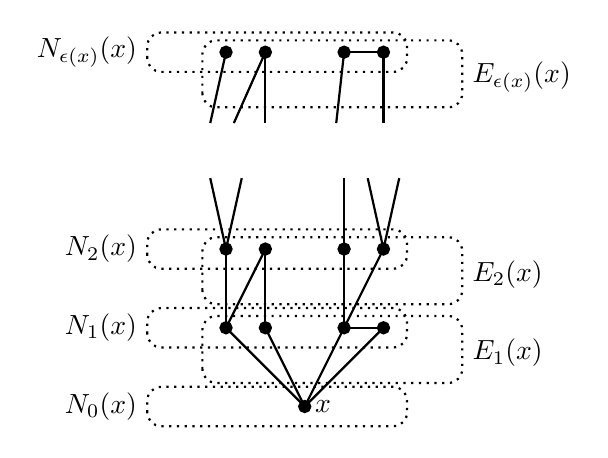
\begin{tikzpicture}[style=thick]
    \coordinate (V0) at (2cm,1cm);
    \coordinate (V11) at (1cm,2cm);
    \coordinate (V12) at (1.5cm,2cm);
    \coordinate (V13) at (2.5cm,2cm);
    \coordinate (V14) at (3cm,2cm);
    \coordinate (V21) at (1cm,3cm);
    \coordinate (V22) at (1.5cm,3cm);
    \coordinate (V23) at (2.5cm,3cm);
    \coordinate (V24) at (3cm,3cm);
    \coordinate (V31) at (0.8cm,3.9cm);
    \coordinate (V32) at (1.2cm,3.9cm);
    \coordinate (V33) at (2.5cm,3.9cm);
    \coordinate (V34) at (2.8cm,3.9cm);
    \coordinate (V35) at (3.2cm,3.9cm);
    \coordinate (V41) at (0.8cm,4.6cm);
    \coordinate (V42) at (1.1cm,4.6cm);
    \coordinate (V43) at (1.5cm,4.6cm);
    \coordinate (V44) at (2.4cm,4.6cm);
    \coordinate (V45) at (3cm,4.6cm);
    \coordinate (Vn1) at (1cm,5.5cm);
    \coordinate (Vn2) at (1.5cm,5.5cm);
    \coordinate (Vn3) at (2.5cm,5.5cm);
    \coordinate (Vn4) at (3cm,5.5cm);
    
    \draw (V0) -- (V11);
    \draw (V0) -- (V12);
    \draw (V0) -- (V13);
    \draw (V0) -- (V14);
    \draw (V13) -- (V14);
    
    \draw (V11) -- (V21);
    \draw (V11) -- (V22);
    \draw (V12) -- (V22);
    \draw (V13) -- (V23);
    \draw (V13) -- (V24);
    
    \draw (V21) -- (V31);
    \draw (V21) -- (V32);
    \draw (V23) -- (V33);
    \draw (V24) -- (V34);
    \draw (V24) -- (V35);
    
    \draw (V41) -- (Vn1);
    \draw (V42) -- (Vn2);
    \draw (V43) -- (Vn2);
    \draw (V44) -- (Vn3);
    \draw (V45) -- (Vn4);
    \draw (Vn3) -- (Vn4);
    
    \draw[dotted,rounded corners=5pt]
  (0,1) node[left]{$N_0(x)$} ++(0,-0.25) rectangle ++(3.3,0.5) ;
  
  \draw[dotted,rounded corners=5pt]
  (0,2) node[left]{$N_1(x)$} ++(0,-0.25) rectangle ++(3.3,0.5) ;
  \draw[dotted,rounded corners=5pt]
  (0.7,1.3) rectangle ++(3.3,0.85) ++(0,-0.47) node[right]{$E_1(x)$};
  
  \draw[dotted,rounded corners=5pt]
  (0,3) node[left]{$N_2(x)$} ++(0,-0.25) rectangle ++(3.3,0.5) ;
  \draw[dotted,rounded corners=5pt]
  (0.7,2.3) rectangle ++(3.3,0.85) ++(0,-0.47) node[right]{$E_2(x)$};
  
  \draw[dotted,rounded corners=5pt]
  (0.7,4.8) rectangle ++(3.3,0.85) ++(0,-0.47) node[right]  {$E_{\epsilon(x)}(x)$} ;
  \draw[dotted,rounded corners=5pt]
  (0,5.5) node[left]{$N_{\epsilon(x)}(x)$} ++(0,-0.25) rectangle ++(3.3,0.5) ;
    
    \draw[fill=black] (V0) circle (2pt) node[right]{$x$};
    \draw[fill=black] (V11) circle (2pt);
    \draw[fill=black] (V12) circle (2pt);
    \draw[fill=black] (V13) circle (2pt);
    \draw[fill=black] (V14) circle (2pt);
    \draw[fill=black] (V21) circle (2pt);
    \draw[fill=black] (V22) circle (2pt);
    \draw[fill=black] (V23) circle (2pt);
    \draw[fill=black] (V24) circle (2pt);
    \draw[fill=black] (Vn1) circle (2pt);
    \draw[fill=black] (Vn2) circle (2pt);
    \draw[fill=black] (Vn3) circle (2pt);
    \draw[fill=black] (Vn4) circle (2pt);
\end{tikzpicture}
\caption{Գագաթների և կողերի տրոհումը ըստ $x$ գագաթից ունեցած հեռավորության}
\label{graphLevels}
\end{figure}
\end{hide}

Այնուհետև ցույց է տրվել, որ Թեորեմ \ref{t2_regular_product}-ի գնահատականը կարելի է էլ ավելի լավացնել, եթե ավելացնենք $G$ գրաֆի ներկման վրա որոշակի պայմաններ: Ֆիքսված $x \in V(G)$ գագաթի համար $G$ կապակցված գրաֆի գագաթների և կողերի բազմությունները տրոհենք մակարդակների՝ ըստ $x$ գագաթից ունեցած հեռավորության.
\begin{center}
$V(G) = \bigcup_{i=0}^{\epsilon(x)}N_i(x)$, որտեղ 
$N_i(x)=\left\{ v \in V(G) : d(v,x)=i \right\}$, $i=0,\ldots,\epsilon(x)$:
\end{center}
Բոլոր $v \in N_i(G)$, $i=1,\ldots,\epsilon(x)$, գագաթների սպեկտրները տրոհենք երկու մասի.
\begin{align*}
S(v,\alpha) &= S_x^-(v,\alpha) \cup S_x^+(v,\alpha),\text{ որտեղ}\\
S_x^-(v,\alpha) &= \left\{ \alpha(vu) : u\in N_{i-1}(x) \cup N_i(x) \right\},\\
S_x^+(v,\alpha) &= \left\{ \alpha(vu) : u\in N_{i+1}(x) \right\}:
\end{align*}

Կասենք, որ $G$ կապակցված գրաֆի $\alpha$ միջակայքային ներկումը \textit{սեպարաբել} է $x$ գագաթի նկատմամբ, եթե ցանկացած $\forall v \in V(G)$ գագաթի համար $\max S_x^-(v,\alpha) < \min S_x^+(v,\alpha)$ (այն դեպքում, երբ $S_x^-(v,\alpha)=\varnothing$, կհամարենք, որ $\max{S_x^-(v,\alpha)}=-\infty$, իսկ երբ $S_x^+(v,\alpha)=\varnothing$, կհամարենք, որ $\min{S_x^+(v,\alpha)}=+\infty$):

\begin{hide}
\begin{figure}[b!]
\centering
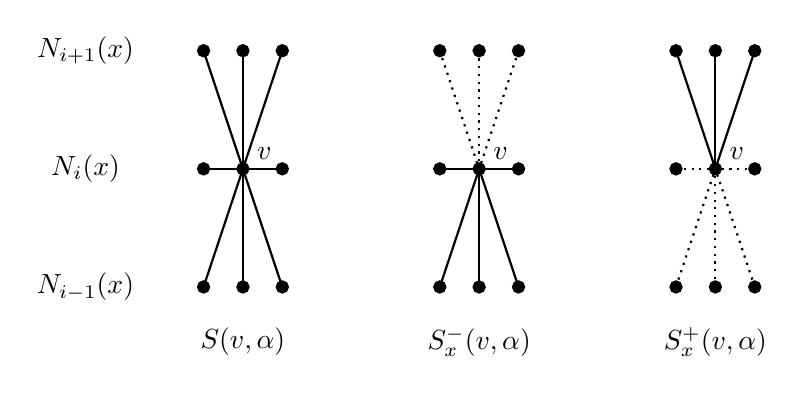
\begin{tikzpicture}[style=thick]
    \node at (-0.5cm, 1cm) {$N_{i-1}(x)$};
    \node at (-0.5cm, 2.5cm) {$N_i(x)$};
    \node at (-0.5cm, 4cm) {$N_{i+1}(x)$};
    
% first sample
    \coordinate (V111) at (1cm,1cm);
    \coordinate (V112) at (1.5cm,1cm);
    \coordinate (V113) at (2cm,1cm);
    \coordinate (V121) at (1cm,2.5cm);
    \coordinate (V122) at (1.5cm,2.5cm);
    \coordinate (V123) at (2cm,2.5cm);
    \coordinate (V131) at (1cm,4cm);
    \coordinate (V132) at (1.5cm,4cm);
    \coordinate (V133) at (2cm,4cm);
    
    \draw (V111) -- (V122);
    \draw (V112) -- (V122);
    \draw (V113) -- (V122);
    \draw (V121) -- (V122);
    \draw (V123) -- (V122);
    \draw (V131) -- (V122);
    \draw (V132) -- (V122);
    \draw (V133) -- (V122);
    
    \draw[fill=black] (V111) circle (2pt);
    \draw[fill=black] (V112) circle (2pt);
    \draw[fill=black] (V113) circle (2pt);
    \draw[fill=black] (V121) circle (2pt);
    \draw[fill=black] (V122) circle (2pt) node[right] at (1.55cm,2.7cm) {$v$};
    \draw[fill=black] (V123) circle (2pt);
    \draw[fill=black] (V131) circle (2pt);
    \draw[fill=black] (V132) circle (2pt);
    \draw[fill=black] (V133) circle (2pt);
    
    \node at (1.5cm, 0.3cm) {$S(v,\alpha)$};
    
% second sample
    \coordinate (V211) at (4cm,1cm);
    \coordinate (V212) at (4.5cm,1cm);
    \coordinate (V213) at (5cm,1cm);
    \coordinate (V221) at (4cm,2.5cm);
    \coordinate (V222) at (4.5cm,2.5cm);
    \coordinate (V223) at (5cm,2.5cm);
    \coordinate (V231) at (4cm,4cm);
    \coordinate (V232) at (4.5cm,4cm);
    \coordinate (V233) at (5cm,4cm);
    
    \draw (V211) -- (V222);
    \draw (V212) -- (V222);
    \draw (V213) -- (V222);
    \draw (V221) -- (V222);
    \draw (V223) -- (V222);
    \draw[dotted] (V231) -- (V222);
    \draw[dotted] (V232) -- (V222);
    \draw[dotted] (V233) -- (V222);
    
    \draw[fill=black] (V211) circle (2pt);
    \draw[fill=black] (V212) circle (2pt);
    \draw[fill=black] (V213) circle (2pt);
    \draw[fill=black] (V221) circle (2pt);
    \draw[fill=black] (V222) circle (2pt) node[right] at (4.55cm,2.7cm) {$v$};
    \draw[fill=black] (V223) circle (2pt);
    \draw[fill=black] (V231) circle (2pt);
    \draw[fill=black] (V232) circle (2pt);
    \draw[fill=black] (V233) circle (2pt);
    
    \node at (4.5cm, 0.3cm) {$S_x^{-}(v,\alpha)$};
    
% third sample
    \coordinate (V311) at (7cm,1cm);
    \coordinate (V312) at (7.5cm,1cm);
    \coordinate (V313) at (8cm,1cm);
    \coordinate (V321) at (7cm,2.5cm);
    \coordinate (V322) at (7.5cm,2.5cm);
    \coordinate (V323) at (8cm,2.5cm);
    \coordinate (V331) at (7cm,4cm);
    \coordinate (V332) at (7.5cm,4cm);
    \coordinate (V333) at (8cm,4cm);
    
    \draw[dotted] (V311) -- (V322);
    \draw[dotted] (V312) -- (V322);
    \draw[dotted] (V313) -- (V322);
    \draw[dotted] (V321) -- (V322);
    \draw[dotted] (V323) -- (V322);
    \draw (V331) -- (V322);
    \draw (V332) -- (V322);
    \draw (V333) -- (V322);
    
    \draw[fill=black] (V311) circle (2pt);
    \draw[fill=black] (V312) circle (2pt);
    \draw[fill=black] (V313) circle (2pt);
    \draw[fill=black] (V321) circle (2pt);
    \draw[fill=black] (V322) circle (2pt) node[right] at (7.55cm,2.7cm) {$v$};
    \draw[fill=black] (V323) circle (2pt);
    \draw[fill=black] (V331) circle (2pt);
    \draw[fill=black] (V332) circle (2pt);
    \draw[fill=black] (V333) circle (2pt);
    
    \node at (7.5cm, 0.3cm) {$S_x^{+}(v,\alpha)$};
    
\end{tikzpicture}
\caption{Գագաթի ստորին և վերին սպեկտրները}
\label{vertexSpectrums}
\end{figure}
\end{hide}


\begin{theorem}
\label{t2_separable}
Դիցուք $G$ կապակցված գրաֆը ունի սեպարաբել միջակայքային $t_G$-ներկում որևէ $x\in V(G)$ գագաթի նկատմամբ, ընդ որում գոյություն ունի $y\in N_{\epsilon(x)}(x)$ գագաթ, որի սպեկտրը պարունակում է $t_G$ գույնը, իսկ $1\in S(x,\alpha)$: Եթե $H$ գրաֆը $r$-համասեռ է և ունի միջակայքային $t_H$-ներկում, ապա
\begin{center}
$W(G \square H) \geq t_G + t_H + \epsilon(x)r$:
\end{center}
\end{theorem}
\begin{proof}[Ապացույց]
Դիցուք $\alpha$-ն $G$-ի սեպարաբել միջակայքային $t_G$-ներկում է $x \in V(G)$ գագաթի նկատմամբ, $\beta$-ն $H$-ի միջակայքային $t_H$-ներկում է: $G \square H$ գրաֆի համար սահմանենք $\gamma$ ներկումը հետևյալ կերպ.

\begin{description}
\item[(1)] $\gamma((x,v)(x,v')) = \beta(vv')$, որտեղ $vv' \in E(H)$,
\item[(2)] $\gamma((u,v)(u,v')) = \beta(vv') + \max{S_x^-(u,\alpha)} + i r$,\\ որտեղ $u\in N_i(x)$, $vv' \in E(H)$ և $i=0,\dots,\epsilon(x)$,
\item[(3)] $\gamma((u,v)(u',v)) = \alpha(uu') + \overline{S}(v,\beta) + i r - r$,\\ որտեղ $uu'\in E_i(x)$, $v \in V(H)$ և $i=1,\dots,\epsilon(x)$:
\end{description}

\begin{hide}
\begin{figure}[t!]
\centering
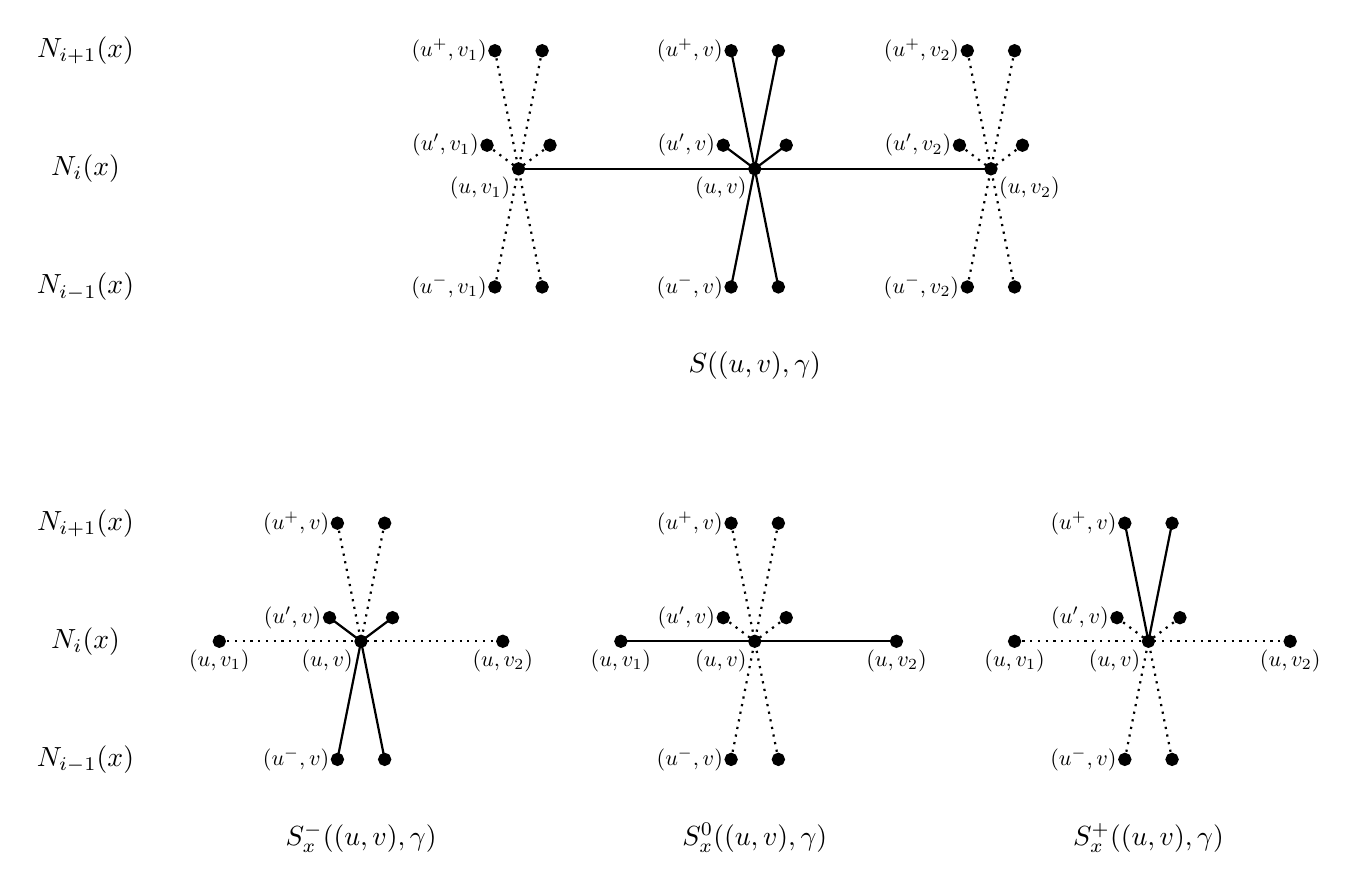
\begin{tikzpicture}[style=thick]
    \node at (-4cm, 1cm) {$N_{i-1}(x)$};
    \node at (-4cm, 2.5cm) {$N_i(x)$};
    \node at (-4cm, 4cm) {$N_{i+1}(x)$};
    \node at (-4cm, 7cm) {$N_{i-1}(x)$};
    \node at (-4cm, 8.5cm) {$N_i(x)$};
    \node at (-4cm, 10cm) {$N_{i+1}(x)$};
    
% whole spectrum
    \coordinate (Va111) at (1.2cm,7cm);
    \coordinate (Va113) at (1.8cm,7cm);
    \coordinate (Va121) at (1.1cm,8.8cm);
    \coordinate (Va122) at (1.5cm,8.5cm);
    \coordinate (Va123) at (1.9cm,8.8cm);
    \coordinate (Va131) at (1.2cm,10cm);
    \coordinate (Va133) at (1.8cm,10cm);
    
    \draw[dotted] (Va111) -- (Va122);
    \draw[dotted] (Va113) -- (Va122);
    \draw[dotted] (Va121) -- (Va122);
    \draw[dotted] (Va123) -- (Va122);
    \draw[dotted] (Va131) -- (Va122);
    \draw[dotted] (Va133) -- (Va122);
    
    \draw[fill=black] (Va111) circle (2pt) node[left,scale=0.8] {$(u^-,v_1)$};
    \draw[fill=black] (Va113) circle (2pt);
    \draw[fill=black] (Va121) circle (2pt) node[left,scale=0.8] {$(u',v_1)$};
    \draw[fill=black] (Va122) circle (2pt) node[below left,scale=0.8] {$(u,v_1)$};
    \draw[fill=black] (Va123) circle (2pt);
    \draw[fill=black] (Va131) circle (2pt) node[left,scale=0.8] {$(u^+,v_1)$};
    \draw[fill=black] (Va133) circle (2pt);
    
    \coordinate (Va211) at (4.2cm,7cm);
    \coordinate (Va213) at (4.8cm,7cm);
    \coordinate (Va221) at (4.1cm,8.8cm);
    \coordinate (Va222) at (4.5cm,8.5cm);
    \coordinate (Va223) at (4.9cm,8.8cm);
    \coordinate (Va231) at (4.2cm,10cm);
    \coordinate (Va233) at (4.8cm,10cm);
    
    \draw (Va211) -- (Va222);
    \draw (Va213) -- (Va222);
    \draw (Va221) -- (Va222);
    \draw (Va223) -- (Va222);
    \draw (Va231) -- (Va222);
    \draw (Va233) -- (Va222);
    
    \draw[fill=black] (Va211) circle (2pt) node[left,scale=0.8] {$(u^-,v)$};
    \draw[fill=black] (Va213) circle (2pt);
    \draw[fill=black] (Va221) circle (2pt) node[left,scale=0.8] {$(u',v)$};
    \draw[fill=black] (Va222) circle (2pt) node[below left,scale=0.8] {$(u,v)$};
    \draw[fill=black] (Va223) circle (2pt);
    \draw[fill=black] (Va231) circle (2pt) node[left,scale=0.8] {$(u^+,v)$};
    \draw[fill=black] (Va233) circle (2pt);
    
    \coordinate (Va311) at (7.2cm,7cm);
    \coordinate (Va313) at (7.8cm,7cm);
    \coordinate (Va321) at (7.1cm,8.8cm);
    \coordinate (Va322) at (7.5cm,8.5cm);
    \coordinate (Va323) at (7.9cm,8.8cm);
    \coordinate (Va331) at (7.2cm,10cm);
    \coordinate (Va333) at (7.8cm,10cm);
    
    \draw[dotted] (Va311) -- (Va322);
    \draw[dotted] (Va313) -- (Va322);
    \draw[dotted] (Va321) -- (Va322);
    \draw[dotted] (Va323) -- (Va322);
    \draw[dotted] (Va331) -- (Va322);
    \draw[dotted] (Va333) -- (Va322);
    
    \draw[fill=black] (Va311) circle (2pt) node[left,scale=0.8] {$(u^-,v_2)$};
    \draw[fill=black] (Va313) circle (2pt);
    \draw[fill=black] (Va321) circle (2pt) node[left,scale=0.8] {$(u',v_2)$};
    \draw[fill=black] (Va322) circle (2pt) node[below right,scale=0.8] {$(u,v_2)$};
    \draw[fill=black] (Va323) circle (2pt);
    \draw[fill=black] (Va331) circle (2pt) node[left,scale=0.8] {$(u^+,v_2)$};
    \draw[fill=black] (Va333) circle (2pt);
    
    % lines between blocks
    \draw (Va122) -- (Va222) -- (Va322);
    
    \node at (4.5cm, 6cm) {$S((u,v),\gamma)$};
    
% spectrum 0    
    \coordinate (Vc211) at (4.2cm,1cm);
    \coordinate (Vc213) at (4.8cm,1cm);
    \coordinate (Vc221) at (4.1cm,2.8cm);
    \coordinate (Vc222) at (4.5cm,2.5cm);
    \coordinate (Vc223) at (4.9cm,2.8cm);
    \coordinate (Vc231) at (4.2cm,4cm);
    \coordinate (Vc233) at (4.8cm,4cm);
    
    \draw[dotted] (Vc211) -- (Vc222);
    \draw[dotted] (Vc213) -- (Vc222);
    \draw[dotted] (Vc221) -- (Vc222);
    \draw[dotted] (Vc223) -- (Vc222);
    \draw[dotted] (Vc231) -- (Vc222);
    \draw[dotted] (Vc233) -- (Vc222);
    
    \draw[fill=black] (Vc211) circle (2pt) node[left,scale=0.8] {$(u^-,v)$};
    \draw[fill=black] (Vc213) circle (2pt);
    \draw[fill=black] (Vc221) circle (2pt) node[left,scale=0.8] {$(u',v)$};
    \draw[fill=black] (Vc222) circle (2pt) node[below left,scale=0.8] {$(u,v)$};
    \draw[fill=black] (Vc223) circle (2pt);
    \draw[fill=black] (Vc231) circle (2pt) node[left,scale=0.8] {$(u^+,v)$};
    \draw[fill=black] (Vc233) circle (2pt);
    
    % neighboring blocks
    \coordinate (Vc322) at (6.3cm,2.5cm);
    \coordinate (Vc122) at (2.8cm,2.5cm);
    \draw[fill=black] (Vc322) circle (2pt) node[below,scale=0.8] {$(u,v_2)$};
    \draw[fill=black] (Vc122) circle (2pt) node[below,scale=0.8] {$(u,v_1)$};
    \draw (Vc122) -- (Vc222) -- (Vc322);
    
    \node at (4.5cm, 0cm) {$S_x^0((u,v),\gamma)$};
    
% spectrum -    
    \coordinate (Vb211) at (-0.8cm,1cm);
    \coordinate (Vb213) at (-0.2cm,1cm);
    \coordinate (Vb221) at (-0.9cm,2.8cm);
    \coordinate (Vb222) at (-0.5cm,2.5cm);
    \coordinate (Vb223) at (-0.1cm,2.8cm);
    \coordinate (Vb231) at (-0.8cm,4cm);
    \coordinate (Vb233) at (-0.2cm,4cm);
    
    \draw (Vb211) -- (Vb222);
    \draw (Vb213) -- (Vb222);
    \draw (Vb221) -- (Vb222);
    \draw (Vb223) -- (Vb222);
    \draw[dotted] (Vb231) -- (Vb222);
    \draw[dotted] (Vb233) -- (Vb222);
    
    \draw[fill=black] (Vb211) circle (2pt) node[left,scale=0.8] {$(u^-,v)$};
    \draw[fill=black] (Vb213) circle (2pt);
    \draw[fill=black] (Vb221) circle (2pt) node[left,scale=0.8] {$(u',v)$};
    \draw[fill=black] (Vb222) circle (2pt) node[below left,scale=0.8] {$(u,v)$};
    \draw[fill=black] (Vb223) circle (2pt);
    \draw[fill=black] (Vb231) circle (2pt) node[left,scale=0.8] {$(u^+,v)$};
    \draw[fill=black] (Vb233) circle (2pt);
    
    % neighboring blocks
    \coordinate (Vb322) at (1.3cm,2.5cm);
    \coordinate (Vb122) at (-2.3cm,2.5cm);
    \draw[fill=black] (Vb322) circle (2pt) node[below,scale=0.8] {$(u,v_2)$};
    \draw[fill=black] (Vb122) circle (2pt) node[below,scale=0.8] {$(u,v_1)$};
    \draw[dotted] (Vb122) -- (Vb222) -- (Vb322);
    
    \node at (-0.5cm, 0cm) {$S_x^-((u,v),\gamma)$};
    
% spectrum +
    \coordinate (Vd211) at (9.2cm,1cm);
    \coordinate (Vd213) at (9.8cm,1cm);
    \coordinate (Vd221) at (9.1cm,2.8cm);
    \coordinate (Vd222) at (9.5cm,2.5cm);
    \coordinate (Vd223) at (9.9cm,2.8cm);
    \coordinate (Vd231) at (9.2cm,4cm);
    \coordinate (Vd233) at (9.8cm,4cm);
    
    \draw[dotted] (Vd211) -- (Vd222);
    \draw[dotted] (Vd213) -- (Vd222);
    \draw[dotted] (Vd221) -- (Vd222);
    \draw[dotted] (Vd223) -- (Vd222);
    \draw (Vd231) -- (Vd222);
    \draw (Vd233) -- (Vd222);
    
    \draw[fill=black] (Vd211) circle (2pt) node[left,scale=0.8] {$(u^-,v)$};
    \draw[fill=black] (Vd213) circle (2pt);
    \draw[fill=black] (Vd221) circle (2pt) node[left,scale=0.8] {$(u',v)$};
    \draw[fill=black] (Vd222) circle (2pt) node[below left,scale=0.8] {$(u,v)$};
    \draw[fill=black] (Vd223) circle (2pt);
    \draw[fill=black] (Vd231) circle (2pt) node[left,scale=0.8] {$(u^+,v)$};
    \draw[fill=black] (Vd233) circle (2pt);
    
    % neighboring blocks
    \coordinate (Vd322) at (11.3cm,2.5cm);
    \coordinate (Vd122) at (7.8cm,2.5cm);
    \draw[fill=black] (Vd322) circle (2pt) node[below,scale=0.8] {$(u,v_2)$};
    \draw[fill=black] (Vd122) circle (2pt) node[below,scale=0.8] {$(u,v_1)$};
    \draw[dotted] (Vd122) -- (Vd222) -- (Vd322);
    
    \node at (9.5cm, 0cm) {$S_x^+((u,v),\gamma)$};
\end{tikzpicture}
\caption{Դեկարտյան արտադրյալի $(u,v)$ գագաթի սպեկտրի տրոհումը}
\label{separable}
\end{figure}
\end{hide}

Ցույց տանք, որ այս ներկման դեպքում բոլոր գագաթների սպեկտրները միջակայքեր են: Յուրաքանչյուր գագաթի սպեկտր տրոհենք 3 չհատվող բազմությունների (Նկ. \ref{separable}).
\begin{center}
$S((u,v),\gamma) = S_x^-((u,v),\gamma) \cup S_x^0((u,v),\gamma) \cup S_x^+((u,v),\gamma) $,
\end{center}
որտեղ
\begin{align*}
S_x^0((u,v),\gamma) &= \left\{ \gamma((u,v)(u,v')) : vv'\in E(H) \right\}, \\
S_x^+((u,v),\gamma) &= \left\{ \gamma((u,v)(u',v)) : uu'\in E_{i+1}(x) \right\}, \\
S_x^-((u,v),\gamma) &= \left\{ \gamma((u,v)(u',v)) : uu'\in E_{i}(x) \right\}, \\
&u \in N_i(x),\ i=0,1,\ldots,\epsilon(x)
\end{align*}


Երբ $u\in N_{\epsilon(x)}(x)$, համարենք, որ $S_x^+((u,v),\gamma)=\varnothing$, իսկ $S_x^-((x,v),\gamma)=\varnothing$:

Հաշվի առնելով, որ $\beta$-ն $H$-ի միջակայքային ներկում է, ըստ $\gamma$ ներկման կառուցման կստանանք.
\begin{align*}
S_x^0((x,v),\gamma) &= \left\{ \beta(vv') | vv'\in E(H) \right\} = [\underline{S}(v,\beta),\overline{S}(v,\beta)]\\
S_x^0((u,v),\gamma) &= \left\{ \beta(vv') + \max{S_x^-(u,\alpha)} + i r : vv'\in E(H) \right\}\\
					&= [\underline{S}(v,\beta) + \max{S_x^-(u,\alpha)} + i r ,\overline{S}(v,\beta) + \max{S_x^-(u,\alpha)} + i r ]
\end{align*}
Քանի որ $\alpha$-ն $G$-ի սեպարաբել միջակայքային ներկում է $x$-ի նկատմամբ՝
\begin{align*}
S_x^+((u,v),\gamma) &= \left\{ \alpha(uu') + \overline{S}(v,\beta) + (i+1)r - r : uu'\in E_{i+1}(x) \right\}\\
					&= [\min{S_x^+(u,\alpha)} + \overline{S}(v,\beta) + i r,\max{S_x^+(u,\alpha)} + \overline{S}(v,\beta) + i r ]\\
S_x^-((u,v),\gamma) &= \left\{ \alpha(uu') + \overline{S}(v,\beta) + i r - r : uu'\in E_{i}(x) \right\}\\
					&= [\min{S_x^-(u,\alpha)} + \overline{S}(v,\beta) + i r - r,\max{S_x^-(u,\alpha)} + \overline{S}(v,\beta) + i r - r ]
\end{align*}
Ըստ թեորեմի պայմանի, $1 \in S(x,\alpha)$: Ուստի՝ $\min{S_x^+(x,\alpha)}=1$, և $\forall v \in V(H)$ գագաթի համար
\begin{center}
$S((x,v),\gamma) = [\underline{S}(v,\beta),\max{S_x^+(x,\alpha)} + \overline{S}(v,\beta)] $
\end{center}
Քանի որ $ \underline{S}(v,\beta) - (\overline{S}(v,\beta) - r) = 1 $ և $ \min{S_x^+(u,\alpha)} - \max{S_x^-(u,\alpha)} = 1$, ստացվում է, որ $\forall u \in V(G),\ u \not= x,\ \forall v \in V(H)$
\begin{center}
$S((u,v),\gamma) = [\min{S_x^-(u,\alpha)} + \overline{S}(v,\beta) + i r - r,\max{S_x^+(u,\alpha)} + \overline{S}(v,\beta) + i r] $:
\end{center}
Այսպիսով, $G\square H$ գրաֆի բոլոր գագաթների սպեկտրները միջակայքեր են: Քանի որ $\beta$-ն $H$-ի միջակայքային $t_H$-ներկում է, $\exists v',v'' \in V(H)$ այնպիսիք, որ $1 \in S(v',\beta)$, $t_H \in S(v'',\beta)$: Մյուս կողմից, ըստ թեորեմի պայմանների՝ $1 \in S(x,\alpha)$ և $t_G \in S(y,\alpha)$, որտեղ $y \in N_{\epsilon(x)}(x)$: Հետևաբար՝
\begin{center}
$1 \in S((x,v'),\gamma)$ և $t_G+t_H+\epsilon(x)r \in S((y,v''),\gamma)$
\end{center}
Ըստ Լեմմա \ref{t1_lemma}-ի՝ $\gamma$-ն $G$ գրաֆի միջակայքային կողային $(t_G+t_H+\epsilon(x)r)$-ներկում է:

\end{proof}

\begin{corollary}
\label{c2_separable_corollary}
Դիցուք $G$-ն հանդիսանում է զույգ երկարությամբ ցիկլ, շղթա, n-չափանի խորանարդ, թրթուրածառ կամ լրիվ երկկողմանի գրաֆ, իսկ $H$-ը միջակայքային ներկելի $r$-համասեռ գրաֆ է: Այդ դեպքում,
\begin{center}
$W(G \square H) \geq W(G) + W(H) + \mathrm{diam}(G)r$:
\end{center}
\end{corollary}

\begin{proof}[Ապացույց]
Այս հետևանքն ապացուցելու համար բավական է ստուգել, որ նշված դասերին պատկանող գրաֆները ունեն առավելագույն թվով գույներով այնպիսի ներկումներ, որոնք բավարարում են Թեորեմ \ref{t2_separable}-ի պայմաններին:

\textbf{1. $\mathbf{G=C_{2n}}$}

Դիցուք, $V(C_{2n})=\left\{x,v_1,\ldots,v_{n-1},y,u_{n-1},\ldots,u_1\right\}$: Այս գրաֆի $W(C_{2n})$-ներկումը տրվում է հետևյալ կերպ.

\bigskip
\begin{tabular}{lll}
$\alpha(xv_1)=1$ & $\alpha(xu_1)=2$ \\
$\alpha(v_iv_{i+1})=i+1$ &$\alpha(u_iu_{i+1})=i+2$ &որտեղ $i=1,\ldots,n-2$\\
$\alpha(v_{n-1}y)=n$ &$\alpha(u_{n-1}y)=n+1$\\
\end{tabular}
\bigskip

Այս դեպքում, եթե գագաթները տրոհենք մակարդակների ըստ $x$ գագաթից ունեցած հեռավորության, ստորին և վերին սպեկտրները կլինեն.

\bigskip
\begin{tabular}{lll}
$S_x^-(v_i,\alpha)=\left\{i\right\}$ &$S_x^+(v_i,\alpha)=\left\{i+1\right\}$ &որտեղ $i=1,\ldots,n-2$\\
$S_x^-(u_i,\alpha)=\left\{i+1\right\}$ &$S_x^+(u_i,\alpha)=\left\{i+2\right\}$ &որտեղ $i=1,\ldots,n-2$\\
\end{tabular}
\bigskip

Այսպիսով,

\bigskip
\begin{tabular}{lll}
$i = \max{S_x^-(v_i,\alpha)} < \min{S_x^+(v_i,\alpha)} = i+1$ &որտեղ $i=1,\ldots,n-2$\\
$i+1 = \max{S_x^-(u_i,\alpha)} < \min{S_x^+(u_i,\alpha)} = i+2$ &որտեղ $i=1,\ldots,n-2$\\
$S_x^+(y,\alpha)=\varnothing$
\end{tabular}
\bigskip

Փաստորեն, $\alpha$ ներկման համար բոլոր գագաթները անջատող են, այսինքն՝ $\alpha$-ն $C_{2n}$-ի սեպարաբել ներկում է: Մյուս կողմից, $1\in S(x,\alpha)$, $W(C_{2n})=n+1 \in S(y,\alpha)$, իսկ $d(x,y)=\epsilon(x)=\mathrm{diam}(C_{2n})=n$: Ուստի, Թեորեմ \ref{t2_separable}-ի բոլոր պայմանները բավարարված են:


\begin{figure}[t!]
\centering
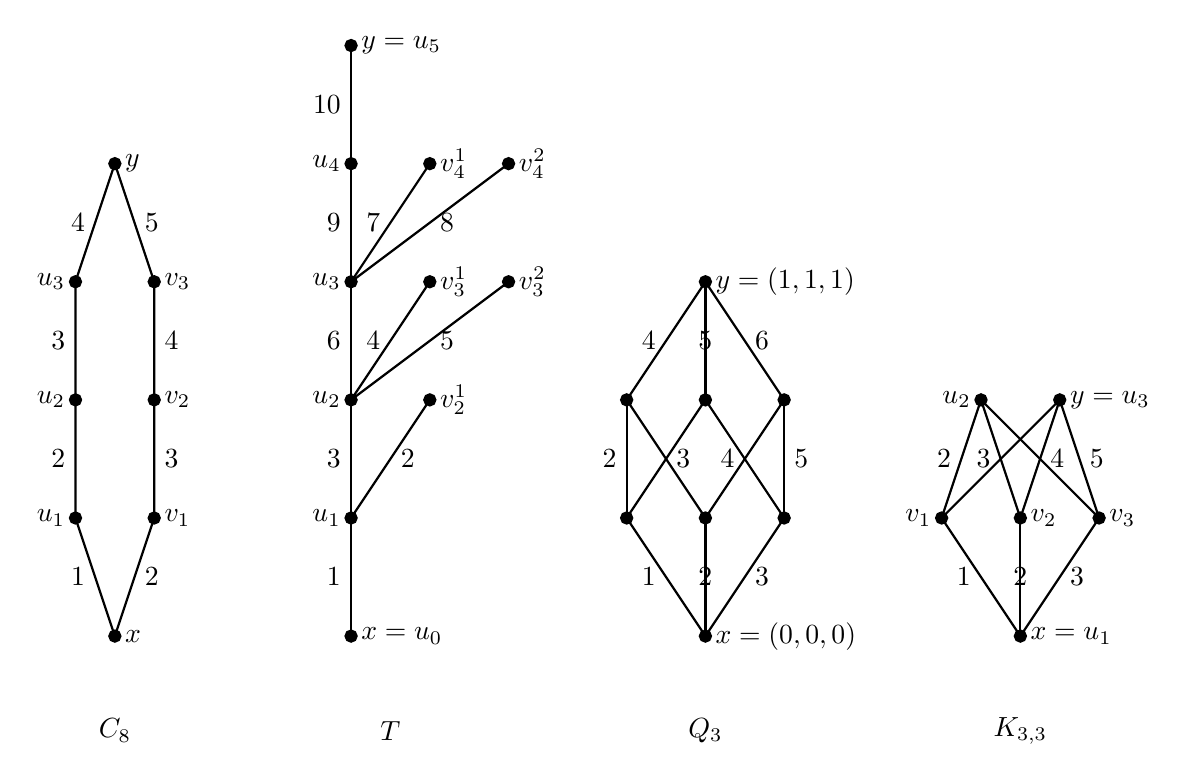
\begin{tikzpicture}[style=thick]
% C_8
    \coordinate (c0) at (-0.5cm,1.5cm);
    \coordinate (c11) at (-1cm,3cm);
    \coordinate (c12) at (-1cm,4.5cm);
    \coordinate (c13) at (-1cm,6cm);
    \coordinate (c21) at (0cm,3cm);
    \coordinate (c22) at (0cm,4.5cm);
    \coordinate (c23) at (0cm,6cm);
    \coordinate (c4) at (-0.5cm,7.5cm);
    
    \draw (c0) -- node[left] {$1$} (c11) 
    -- node[left] {$2$} (c12) 
    -- node[left] {$3$} (c13) 
    -- node[left] {$4$} (c4);
    \draw (c0) -- node[right] {$2$} (c21) 
    -- node[right] {$3$} (c22) 
    -- node[right] {$4$} (c23) 
    -- node[right] {$5$} (c4);
    
    \draw[fill=black] (c0) circle (2pt)  node[right] {$x$};
    \draw[fill=black] (c11) circle (2pt) node[left] {$u_1$};
    \draw[fill=black] (c12) circle (2pt) node[left] {$u_2$};
    \draw[fill=black] (c13) circle (2pt) node[left] {$u_3$};
    \draw[fill=black] (c21) circle (2pt) node[right] {$v_1$};
    \draw[fill=black] (c22) circle (2pt) node[right] {$v_2$};
    \draw[fill=black] (c23) circle (2pt) node[right] {$v_3$};
    \draw[fill=black] (c4) circle (2pt) node[right] {$y$};
    
    \node at (-0.5cm, 0.3cm) {$C_8$};
    
% Caterpillar
    \coordinate (t0) at (2.5cm,1.5cm);
    \coordinate (t1) at (2.5cm,3cm);
    \coordinate (t21) at (2.5cm,4.5cm);
    \coordinate (t22) at (3.5cm,4.5cm);
    
    \coordinate (t31) at (2.5cm,6cm);
    \coordinate (t32) at (3.5cm,6cm);
    \coordinate (t33) at (4.5cm,6cm);
    
    \coordinate (t41) at (2.5cm,7.5cm);
    \coordinate (t42) at (3.5cm,7.5cm);
    \coordinate (t43) at (4.5cm,7.5cm);
    
    \coordinate (t5) at (2.5cm,9cm);
    
    \draw (t0) -- node[left] {$1$} (t1);
    \draw (t1) -- node[left] {$3$} (t21);
    \draw (t1) -- node[right] {$2$} (t22);
    \draw (t21) -- node[left] {$6$} (t31);
    \draw (t21) -- node[left] {$4$} (t32);
    \draw (t21) -- node[right] {$5$} (t33);
    \draw (t31) -- node[left] {$9$} (t41);
    \draw (t31) -- node[left] {$7$} (t42);
    \draw (t31) -- node[right] {$8$} (t43);
    \draw (t41) -- node[left] {$10$} (t5);
    
    \draw[fill=black] (t0) circle (2pt)  node[right] {$x=u_0$};
    \draw[fill=black] (t1) circle (2pt) node[left] {$u_1$};
    \draw[fill=black] (t21) circle (2pt) node[left] {$u_2$};
    \draw[fill=black] (t22) circle (2pt) node[right] {$v_2^1$};
    \draw[fill=black] (t31) circle (2pt) node[left] {$u_3$};
    \draw[fill=black] (t32) circle (2pt) node[right] {$v_3^1$};
    \draw[fill=black] (t33) circle (2pt) node[right] {$v_3^2$};
    \draw[fill=black] (t41) circle (2pt) node[left] {$u_4$};
    \draw[fill=black] (t42) circle (2pt) node[right] {$v_4^1$};
    \draw[fill=black] (t43) circle (2pt) node[right] {$v_4^2$};
    \draw[fill=black] (t5) circle (2pt)  node[right] {$y=u_5$};
    
    \node at (3cm, 0.3cm) {$T$};
    
    
% Q_3
    \coordinate (q000) at (7cm,1.5cm);
    \coordinate (q100) at (6cm,3cm);
    \coordinate (q010) at (7cm,3cm);
    \coordinate (q001) at (8cm,3cm);
    
    \coordinate (q110) at (6cm,4.5cm);
    \coordinate (q101) at (7cm,4.5cm);
    \coordinate (q011) at (8cm,4.5cm);
    \coordinate (q111) at (7cm,6cm);
    
    \draw (q000) -- node[left] {$1$} (q100);
    \draw (q000) -- node {$2$} (q010);
    \draw (q000) -- node[right] {$3$} (q001);
    
    \draw (q100) -- node[left] {$2$} (q110);
    \draw (q100) --  (q101);
    \draw (q010) -- node[right] {$3$} (q110);
    \draw (q010) --  (q011);
    \draw (q001) -- node[left] {$4$} (q101);
    \draw (q001) -- node[right] {$5$} (q011);
    
    \draw (q110) -- node[left] {$4$} (q111);
    \draw (q101) -- node {$5$} (q111);
    \draw (q011) -- node[right] {$6$} (q111);
    
    \draw[fill=black] (q000) circle (2pt)  node[right] {$x=(0,0,0)$};
    \draw[fill=black] (q100) circle (2pt);  
    \draw[fill=black] (q010) circle (2pt);  
    \draw[fill=black] (q001) circle (2pt);  
    \draw[fill=black] (q110) circle (2pt);  
    \draw[fill=black] (q101) circle (2pt);  
    \draw[fill=black] (q011) circle (2pt);  
    \draw[fill=black] (q111) circle (2pt) node[right] {$y=(1,1,1)$};  
    
    \node at (7cm, 0.3cm) {$Q_3$};
    
    
% K_3,3
    \coordinate (b0) at (11cm,1.5cm);
    \coordinate (b11) at (10cm,3cm);
    \coordinate (b12) at (11cm,3cm);
    \coordinate (b13) at (12cm,3cm);
    
    \coordinate (b21) at (10.5cm,4.5cm);
    \coordinate (b22) at (11.5cm,4.5cm);
    
    \draw (b0) -- node[left] {$1$} (b11);
    \draw (b0) -- node {$2$} (b12);
    \draw (b0) -- node[right] {$3$} (b13);
    
    \draw (b11) -- node[left] {$2$} (b21);
    \draw (b11) -- node[left] {$3$} (b22);
    \draw (b12) --  (b21);
    \draw (b12) --  (b22);
    \draw (b13) -- node[right] {$4$} (b21);
    \draw (b13) -- node[right] {$5$} (b22);
    
    \draw[fill=black] (b0) circle (2pt)  node[right] {$x=u_1$};
    \draw[fill=black] (b11) circle (2pt)  node[left] {$v_1$};  
    \draw[fill=black] (b12) circle (2pt)  node[right] {$v_2$};  
    \draw[fill=black] (b13) circle (2pt)  node[right] {$v_3$};  
    \draw[fill=black] (b21) circle (2pt)  node[left] {$u_2$};  
    \draw[fill=black] (b22) circle (2pt)  node[right] {$y=u_3$};  
    
    \node at (11cm, 0.3cm) {$K_{3,3}$};
    
    
\end{tikzpicture}
\caption{$C_8$-ի, թրթուրածառի, $Q_3$-ի և $K_{3,3}$-ի սեպարաբել ներկումները}
\label{separableExamples}
\end{figure}

\bigskip

\textbf{2. $\mathbf{G=T}$, $T$-ն թրթուրածառ է}

Դիցուք $T$-ի գագաթների բազմությունը հետևյալն է.
\begin{center}
$V(T) = \left\{u_0,u_1,v_1^1,\ldots,v_1^{k_1},u_2,v_2^1,\ldots,v_2^{k_2},\ldots,u_{n-1},v_{n-1}^1,\ldots,v_{n-1}^{k_n},u_n\right\}$
\end{center}
որտեղ $n\geq 1$, $k_i\geq 0$, $i=1,\ldots,n-1$: Թրթուրածառի կողերի բազմությունը կլինի՝
\begin{center}
$E(T) = \left\{u_iu_{i+1} : i=0,\ldots,n-1\right\} \cup \left\{u_iv_i^j : i=1,\ldots,n-1,j=1,\ldots,k_i\right\}$
\end{center}
$T$-ի $\beta$ միջակայքային կողային ներկումը տրվում է հետևյալ կերպ.
\begin{center}
\begin{tabular}{lll}
$\beta(u_iu_{i+1}) = \sum\limits_{s=1}^{i}{k_s}+i+1$ &որտեղ $i=0,\ldots,n-1$ \\
$\beta(u_iv_i^j) = \sum\limits_{s=1}^{i-1}{k_s}+i+j$ &որտեղ $i=1,\ldots,n-1$, $j=1,\ldots,k_i$ \\
\end{tabular}
\end{center}
Տրոհենք $T$-ի գագաթներն ու կողերը մակարդակների ըստ $u_0$ գագաթից ունեցած հեռավորության: Այս դեպքում վերին և ստորին սպեկտրները կլինեն.
\begin{center}
\begin{tabular}{lll}
$S_{u_0}^-(u_i,\beta) = \left\{\sum\limits_{s=1}^{i}{k_s}+i+1\right\}$ &որտեղ $i=1,\ldots,n$ \\
$S_{u_0}^+(u_i,\beta) = \left[\sum\limits_{s=1}^{i-1}{k_s}+i+1,\sum\limits_{s=1}^{i}{k_s}+i+1\right]$ &որտեղ $i=0,\ldots,n-1$ \\
$S_{u_0}^-(v_i^j,\beta) = \left\{\sum\limits_{s=1}^{i-1}{k_s}+i+j\right\}$ &որտեղ $i=0,\ldots,n-1$, $j=1,\ldots,k_i$ \\
$S_{u_0}^+(v_i^j,\beta) = \varnothing$, $S_{u_0}^+(u_n,\beta) = \varnothing$
\end{tabular}
\end{center}
Ուստի, բոլոր գագաթները անջատող են $u_0$ գագաթի նկատմամբ: Մյուս կողմից՝
\begin{center}
\begin{tabular}{lll}
$1 \in S(u_0,\beta)$\\
$\sum\limits_{s=1}^{n-1}{k_s}+n=|E(T)|=W(T) \in S(u_n,\beta)$ \\
$d_T(u_0,u_n)=n=\mathrm{diam}(T)$\\
\end{tabular}
\end{center}
Հետևաբար, բավարարված են Թեորեմ \ref{t2_separable}-ի բոլոր պայմանները:

\bigskip

\textbf{3. $\mathbf{G=P_n}$} \\
Նկատենք, որ $P_n$ շղթան թրթուրածառի մասնավոր դեպքն է, երբ 
\begin{center}
$k_1=\ldots=k_{n-1}=0$:
\end{center}
Ուստի այս դեպքի ապացույցը բխում է նախորդ կետից:

\bigskip

\textbf{4. $\mathbf{G=K_{m,n}}$}
\begin{align*}
V(K_{m,n}) &= \left\{u_1,\ldots,u_m,v_1,\ldots,v_n\right\} \\
E(K_{m,n}) &= \left\{u_iv_j : i=1,\ldots,m,\ j=1,\ldots,n\right\}
\end{align*}
$K_{m,n}$-ի $\gamma$ միջակայքային ներկումը տրվում է հետևյալ կերպ.
\begin{center}
$\gamma(u_iv_j)=i+j-1$
\end{center}
Գագաթների և կողերի բազմությունները տրոհենք ըստ $u_1$ գագաթից ունեցած հեռավորության: Գագաթների ստորին և վերին սպեկտրները կլինեն՝
\begin{center}
\begin{tabular}{lll}
$S_{u_1}^-(v_j,\gamma)=\left\{ \gamma(u_1v_j) \right\} = \left\{ j \right\}$ &որտեղ $j=1,\ldots,n$ \\
$S_{u_1}^+(v_j,\gamma)=\left\{ \gamma(v_ju_i) | i=2,\ldots,m \right\} = \left[j+1,j+m-1 \right]$ &որտեղ $j=1,\ldots,n$ \\
$S_{u_1}^+(u_i,\gamma)=\varnothing$ &որտեղ $i=2,\ldots,m$
\end{tabular}
\end{center}
Այսպիսով, բոլոր գագաթները անջատող են $u_1$-ի նկատմամբ և
\begin{center}
\begin{tabular}{lll}
$1 \in S(u_1,\gamma)$\\
$m+n-1=W(K_{m,n}) \in S(u_m,\gamma)$ \\
$d_{K_{m,n}}(u_1,u_m)=2=\mathrm{diam}(K_{m,n})$\\
\end{tabular}
\end{center}
Թեորեմ \ref{t2_separable}-ի բոլոր պայմանները բավարարված են:

\bigskip

\textbf{5. $\mathbf{G=Q_n}$}
\begin{center}
$V(Q_n)=\left\{(b_1,\ldots,b_n) | b_i \in \left\{0,1\right\}\right\}$
\end{center}
$n$-չափանի խորանարդի $\alpha$ միջակայքային $\frac{1}{2}n(n+1)$-ներկումը տրվել է \cite{Petrosyan2010}-ում, իսկ \cite{PetrosyanKhachatrianYepremyanTananyan2011,PetrosyanKhachatrianTananyan2013}-ում ապացուցվել է, որ ավելի շատ գույներ օգտագործող ներկում գոյություն չունի: Այդ ներկման կառուցման ալգորիթմից հետևում է, որ այն սեպարաբել է, ընդ որում՝ 
\begin{center}
\begin{tabular}{lll}
$1 \in S((0,\ldots,0),\alpha)$\\
$\frac{1}{2}n(n+1)=W(Q_n) \in S((1,\ldots,1),\alpha)$ \\
$d_{Q_n}((0,\ldots,0),(1,\ldots,1))=n=\mathrm{diam}(Q_n)$\\
\end{tabular}
\end{center}
Ուստի Թեորեմ \ref{t2_separable}-ի բոլոր պայմանները այս դեպքում ևս բավարարվում են:
\end{proof}
